\documentclass[
    ngerman,
    a4paper,
    11pt
]{report}

\usepackage[utf8]{inputenc}
\usepackage[ngerman]{babel}

\usepackage{fancyhdr}

\usepackage{syntax}

\usepackage{algorithm}
\usepackage{algpseudocode}

\usepackage{parskip}
\usepackage{csquotes}
\usepackage{mdframed}

\usepackage{titlesec}
\titleformat{\chapter}[hang]
  {\normalfont\huge\bfseries}{\thechapter}{10pt}{}

\usepackage[
	hyperref=true,
    bibencoding=inputenc,
    backend=bibtex,
    style=numeric,
	sorting=nty]{biblatex}

\usepackage{hyperref}
\usepackage{amsmath}
\usepackage{cleveref}

\usepackage[toc]{appendix}

\crefname{listing}{Quellcode}{Quellcode}
\crefname{algorithm}{Algorithmus}{Algorithmus}
\usepackage{graphicx}

\usepackage[chapter]{minted}
\usepackage{xcolor}

\usepackage{acronym}

\renewcommand\listingscaption{Quellcode}
\renewcommand\listoflistingscaption{Quellcodeverzeichnis}
\renewcommand{\appendixtocname}{Anhang}

\floatname{algorithm}{Algorithmus}

\bibliography{bericht}

\newcommand{\rust}[1]{\mintinline{rust}{#1}}
\newcommand{\asm}[1]{\mintinline{gas}{#1}}
\newcommand{\ts}[1]{\mintinline{typescript}{#1}}

\newcommand{\Emu}{WIP} % Name des Emulators

\newcommand{\Autor}{Felix Hirschel, Moritz Gutfleisch und Nico Thomas}
\author{Hirschel, Felix \and Gutfleisch, Moritz \and Thomas, Nico}
\newcommand{\MatrikelNummer}{4711}
\newcommand{\Kursbezeichnung}{Tinf19B1, Tinf19B4}

\newcommand{\Titel}{\Emu: WebAssembly-basierter Intel 8080 Emulator}
\newcommand{\AbgabeDatum}{1. April 2090}

\newcommand{\Dauer}{30 Wochen}

\newcommand{\Abschluss}{Bachelor of Science}

\newcommand{\Studiengang}{Informatik}

\newcommand{\Was}{Studienarbeit }

\newcommand{\FirmenName}{SAP SE, Siemens AG}
\newcommand{\FirmenStadt}{Walldorf, Karlsruhe}

\newcommand{\BetreuerDHBW}{Prof. Dr. Kai Becher}

\hypersetup{%%
  pdfauthor={\Autor},
  pdftitle={\Titel},
  pdfsubject={\Was}
}

\pagestyle{fancy}

\rhead{\leftmark}
\lhead{\Emu}

\newcommand{\zB}{z.\,B. }   % "z.B." mit kleinem Leeraum dazwischen (ohne wäre nicht korrekt)
\newcommand{\dash}{d.\,h. }

\newcommand{\code}[1]{\texttt{#1}} % Ist einfacher zu schreiben als ständig \texttt und erlaubt

\newcommand{\regex}[1]{\ensuremath{
  \begingroup
  \makeord{+}
  \makeord{*}
  \makeord{?}
  #1
  \endgroup
}}

\makeatletter
\newcommand{\makeord}[1]{
  \@tempcnta=\mathcode`#1
  \divide\@tempcnta by "1000
  \multiply\@tempcnta by "1000
  \mathcode`#1=\numexpr\the\mathcode`#1-\@tempcnta\relax
}
\makeatother

\makeatletter
\renewenvironment{abstract}{%
  \if@twocolumn
    \section*{\abstractname}%
  \else
    \small
    \begin{center}%
      {\bfseries \abstractname\vspace{-.5em}\vspace{\z@}}%
    \end{center}%
    \quotation
  \fi}
  {\if@twocolumn\else\endquotation\fi}
\makeatother

%\crefname{code}{Auflistung}{Auflistungen}

\begin{document}
\pagenumbering{Roman}

%\begin{titlepage}
\thispagestyle{empty}
\begin{center}
\vspace*{-2cm}
\hfill
\includegraphics[width=4cm]{dhbw-logo}\\[2cm]
{\Huge \Titel}\\[1cm]
{\Huge\scshape \Was}\\[1cm]
{\large für die Prüfung zum}\\[0.5cm]
{\Large \Abschluss}\\[0.5cm]
{\large des Studienganges \Studiengang}\\[0.5cm]
{\large an der}\\[0.5cm]
{\large Dualen Hochschule Baden-Württemberg Karlsruhe}\\[0.5cm]
{\large von}\\[0.5cm]
{\large\bfseries \Autor}\\[1cm]
{\large Abgabedatum \AbgabeDatum}
\vfill
\end{center}
\begin{tabular}{l@{\hspace{2cm}}l}
Bearbeitungszeitraum	         & \Dauer 			\\
Matrikelnummer	                 & \MatrikelNummer		\\
Kurs			         & \Kursbezeichnung		\\
Ausbildungsfirma	         & \FirmenName			\\
Gutachter der Studienakademie	 & \BetreuerDHBW		\\
\end{tabular}
%\end{titlepage}

%%%%%%%%%%%%%%%%%%%%%%%%%%%%%%%%%%%%%%%%%%%%%%%%%%%%%%%%%%%%%%%%%%%%%%%%%%%%%%%
%% Descr:       Vorlage für Berichte der DHBW-Karlsruhe, Erklärung
%% Author:      Prof. Dr. Jürgen Vollmer, vollmer@dhbw-karlsruhe.de
%% $Id: erklaerung.tex,v 1.11 2020/03/13 14:24:42 vollmer Exp $
%% -*- coding: utf-8 -*-
%%%%%%%%%%%%%%%%%%%%%%%%%%%%%%%%%%%%%%%%%%%%%%%%%%%%%%%%%%%%%%%%%%%%%%%%%%%%%%%

% In Bachelorarbeiten muss eine schriftliche Erklärung abgegeben werden.
% Hierin bestätigen die Studierenden, dass die Bachelorarbeit, etc.
% selbständig verfasst und sämtliche Quellen und Hilfsmittel angegeben sind. Diese Erklärung
% bildet das zweite Blatt der Arbeit. Der Text dieser Erklärung muss auf einer separaten Seite
% wie unten angegeben lauten.

\newpage
\thispagestyle{empty}
\begin{framed}
\begin{center}
\Large\bfseries Erklärung
\end{center}
\medskip
\noindent
% siehe §5(3) der \enquote{Studien- und Prüfungsordnung DHBW Technik} vom 29.\,9.\,2017 und Anhang 1.1.13
Wir versichern hiermit, dass wir unsere \Was mit dem Thema:
\enquote{\Titel}
selbstständig verfasst und keine anderen als die angegebenen Quellen und Hilfsmittel benutzt haben. Wir versicheren zudem, dass die eingereichte elektronische Fassung mit der gedruckten Fassung übereinstimmt.
\vskip 1cm
\noindent\begin{tabular}{ll}
\makebox[2.5in]{\hrulefill} & \makebox[2.0in]{\hrulefill}\\
Ort~~~~~Datum & Unterschrift\hspace{4cm}\\[6ex]
\makebox[2.5in]{\hrulefill} & \makebox[2.0in]{\hrulefill}\\
Ort~~~~~Datum & Unterschrift\hspace{4cm}\\[6ex]
\makebox[2.5in]{\hrulefill} & \makebox[2.0in]{\hrulefill}\\
Ort~~~~~Datum & Unterschrift\hspace{4cm}\\
\end{tabular}
%\underline{\hspace{4cm}}\hfill\underline{\hspace{6cm}}\\
\end{framed}

%%%%%%%%%%%%%%%%%%%%%%%%%%%%%%%%%%%%%%%%%%%%%%%%%%%%%%%%%%%%%%%%%%%%%%%%%%%%%%%
\endinput
%%%%%%%%%%%%%%%%%%%%%%%%%%%%%%%%%%%%%%%%%%%%%%%%%%%%%%%%%%%%%%%%%%%%%%%%%%%%%%%

\thispagestyle{empty}

\begin{abstract}
\noindent
Die vorliegende Studienarbeit befasst sich mit der Emulation des 8-Bit-Mikroprozessors Intel 8080 in Rust. Neben einer Simulation des Verhaltens der Hardware gab es den Anspruch an die Bereitstellung einer Entwicklungsumgebung, mit welcher der Prozessor benutzt werden kann. Im Zuge dessen wurden neben dem Emulator eine Weboberfläche, bestehend aus Code-Editor und Visualisierung des Speichers entwickelt. Die Verbindung zwischen geschriebenem Code und dem Emulator bildet ein zusätzlich entwickelter Assembler, der entsprechenden Bytecode generiert.

Wissenschaftlicher Anspruch dieser Arbeit ist eine erstmalige programmatische Umsetzung des Intel 8080 in Kombination von Rust und WebAssembly. Neben ausführlichen Erläuterungen des entwickelten Emulators, wird dieser im Bezug auf Korrektheit und Performanz evaluiert.
\end{abstract}



\tableofcontents

\listoftables
\addcontentsline{toc}{section}{Tabellenverzeichnis}
\listoflistings
\addcontentsline{toc}{section}{Quellcodeverzeichnis}
\chapter*{Abkürzungsverzeichnis}
\addcontentsline{toc}{section}{Abkürzungsverzeichnis}

\begin{acronym}[CPM]
    \acro{ALU}{Arithmetic Logic Unit}
    \acro{API}{Application Programming Interface}
    \acro{BDOS}{Basic Disk Operating System}
    \acro{CPM}[CP/M]{Control Program for Microcomputers}
    \acro{CPU}{Central Processing Unit}
    \acro{CRC}{Cyclic Redundancy Check}
    \acro{EBNF}{Erweiterte Backus-Naur-Form}
    \acro{LIFO}{Last In-First Out}
    \acro{PC}{Program Counter}
    \acro{PSW}{Program Status Word}
    \acro{RAM}{Arbeitsspeicher}
    \acro{SP}{Stack Pointer}
    \acro{SPA}{Single-Page-Applikation}
    \acro{WASM}[Wasm]{WebAssembly}
    \acro{WIP}{WebAssembly Intel 8080 Processor}
\end{acronym}

\acrodefplural{SPA}[SPA]{Single-Page-Applikationen}


\clearpage
\pagenumbering{arabic}
\chapter{Einleitung}

Zu sagen Maschinensprache sei allgegenwärtig ist für nicht-Informatiker eine Aussage, mit der vermutlich zuerst nicht viel angefangen werden kann. Schließlich erfolgt der Kontakt mit den meisten elektronischen Geräten im Alltag entweder durch ein Touch Panel oder unterschiedliche Formen von Schaltern und Knöpfen, keine Eingabe von Nullen und Einsen. Wird sich länger mit der Thematik befasst, muss man feststellen, dass letzten Endes alle diese Interfaces nur eine Abstraktion darstellen. Keins steuert unmittelbar das Verhalten des darunterliegenden Systems insofern, dass ein System PC wüsste, was bspw. \glqq drucke Dokument\grqq{} bedeutet.

Damit Steuerungsanweisungen für elektronische Systeme verständlich werden, müssen diese in Zahlen vorliegen und zusätzlich müssen diese Zahlen interpretiert werden können. Schließlich handelt es sich um keine natürliche Form der Information. Die Interpretation geschieht seither mithilfe einer \ac{CPU}. Diese ist dazu in der Lage numerische Daten in Befehle umzusetzen und ein System mittels der Belegung von Pins, an die eventuelle Ein- und Ausgabegeräte angeschlossen sind, zu steuern.

In der heutigen Zeit gibt es nur noch für wenige Entwickler den Bedarf direkt auf die \ac{CPU} zuzugreifen, höherlevelige Sprachen vereinfachen den Zugriff soweit, dass die Informationsdarstellung dem Menschen in den meisten Fällen verständlich bleibt. Um ein tieferes Verständnis von der grundlegenden Funktionsweise digitaler Systeme zu erhaletn, bietet es sich trotzdem an, einmal mit Assembler, der Sprache am nähesten an Maschinensprache, zu arbeiten.
\medskip

Durch die Leistung heutiger PCs ist zur Ausführung von Maschinencode (zu bspw. Lernzwecken) keine zusätzliche \ac{CPU} in Hardware mehr notwendig. Stattdessen lässt sich deren Verhalten, je nach benötigter Leistung des gewünschten Systems, mit modernen Prozessoren simulieren. Vorliegende Arbeit befasst sich mit eben dieser Simulation eines älteren Mikroprozessors, dem Intel 8080.

Die Wahl fiel deshalb auf den Intel 8080, weil dieser als \glqq Einsteigerprozessor\grqq{} bekannt ist, sich also einerseits für Entwickler eignet, die erste Berührpunkte mit der Entwicklung auf Systemebene suchen, andererseits für die, die sich nocht nicht in großem Maß mit der Emulation solcher Systeme befasst haben. Der Ruf rührt vor allem daher, dass eine umfangreiche Dokumentation vorhanden ist und es sich um ein 8-Bit-System handelt, das eine überschaubare Menge an Befehlen unterstützt. Die genaue Funktionsweise und Eigenheiten werden in Kapitel \ref{chap:basics:intel8080} näher ausgeführt.

Wie später im Kapitel \glqq Verwandte Arbeiten\grqq{} (\ref{chap:similar-work}) dargestellt, gibt es auf dem Gebiet der Emulation bereits eine Vielzahl von Arbeiten, umgesetzt in den verschiedensten digitalen Ökosystemen. Die Simulation ist vor allem unter dem Aspekt interessant, einen tieferen Einblick in die Funktionsweise solcher Systeme, die Vorreiter unserer heutigen Generation von PCs sind, zu erhalten. Deshalb soll nicht nur der Prozessor als solcher emuliert werden, es soll auch eine Oberfläche entwickelt werden, die dem Anwender den Systemzustand zeigt und es ermöglicht eigenen Assemblercode zu schreiben, der so nah am Maschinencode wie möglich ist. Ein systematischer Aufbau der kompletten Anwendung ist in Kapitel \ref{chap:design} zu finden. Auf diesem basiert der Schwerpunkt der Arbeit, die Implementierung in Kapitel \ref{chap:impl}.

\chapter{Grundlagen}\label{chap:prereqs}

\section{WebAssembly}

"\ac{WASM} is a safe, portable, low-level code format designed for efficient execution and compact representation"\cite{WebAssemblyCoreSpecification}. Im Endeffekt handelt es sich bei \ac{WASM} also um eine low-level Bytecode-Sprache, die von Browsern ausgeführt werden kann. Diese Sprache soll ähnlich performant sein, wie die Ausführung naives Maschinen-Codes. Das Paper, in dem \ac{WASM} eingeführt wird, berichtet eine 10\% Performance-Diskrepanz zwischen \ac{WASM} und naivem Assembly\cite{10.1145/3062341.3062363}. Durch Kompilation nach \ac{WASM} ist es möglich Programme auf Seite des Clienten laufen zu lassen, die sonst vom Server ausgeführt werden müssten.
Für viele Programmiersprachen gibt es entsprechende Compiler, die es ermöglichen nach \ac{WASM} zu übersetzen (bspw. C/C++, Rust, usw.).

In der entsprechenden Sprache muss explizit die Schnittstelle zu JavaScript deklariert werden, um festzulegen welche Funktionalitäten dem Frontend zur Verfügung stehen.

\section{Rust}

Rust ist eine moderne, performante, speichersichere Programmiersprache\footnote{siehe \url{https://www.rust-lang.org/} für mehr}. Rust's Sprachmodell verhindert die meisten Laufzeitfehler schon zur Compilezeit, wodurch die Entwicklung deutlich angenehmer wird als bei vergleichbaren Sprachen (bspw. C/C++). Außerdem eignet sich Rust aufgrund der umfassenden Dokumentation sehr gut für \ac{WASM}-Anwendungen\footnote{siehe \url{https://rustwasm.github.io/docs/book/}}.

In diesem Abschnitt werden einige grundlegende Sprachkonstrukte/-konzepte erläutert, die nützlich zum Verständnis dieser Arbeit sind.
Diese Informationen stammen direkt aus der offiziellen Dokumentation: Dem Rust Book \cite{rustBook} und der Dokumentation der Standard-Library \cite{rustDoc}.

\subsection{Structs}

Klassen der Objektorientierung werden in Rust mithilfe von sog. \glqq Structs\grqq{} (Structures) realisiert. Dabei handelt es sich um eigens definierbare Datentypen die über einen Namen mehrere Attribute zusammenfassen. Die Definition eines solchen Structs ist im Folgenden zu sehen. Sie sind Grundlage für die Entwicklung in der vorliegenden Arbeit, die primär auf objektorientierten Ansätzen aufbaut.

\begin{minted}{rust}
    struct Example {
        name: String,
	    valid: bool,
    }
    let ex = Example { name: String::from("Name"), valid: true};
\end{minted}


Wie im Beispielcode zu sehen, befinden sich in der Definition des Structs \rust{Example} keine Methoden. Das liegt daran, dass diese nicht an dieser Stelle stehen dürfen. Stattdessen geschieht dies mittels einem eigenen \glqq Implementation Block\grqq. Dieser lässt sich mittels \rust{impl Example { }} definieren. In diesem Block können nach belieben Methoden implementiert werden, die dann vom entsprechenden Struct zur Verfügung gestellt werden. 

Bei ihrer Implementierung sind Methoden implizit von privatem Scope, können also nur innerhalb der \rust{.rs}-Datei genutzt werden, in der sie beschrieben sind. Das Schlüsselwort \rust{pub} erlaubt es auch in anderen Dateien entsprechende Methoden zu verwenden. Methoden die innerhalb eines mit \rust{impl} geöffneten Blocks stehen beziehen sich immer auf einen Struct und können mittels dem \rust{&self}-Objekt auf die entsprechende Instanz und deren Felder zugreifen.

\subsection{Traits}

Mithilfe von Traits lässt sich in Rust das Verhalten von Structs (oder allgemeiner: Typen) definieren. Die Analogie zu herkömmlichen Sprachen ist das \textit{Interface}. Genau wie diese definieren Structs eine oder mehrere Funktionalitäten, die der Compiler bei einem Objekt erwarten kann. Ihre Definition sieht ebenfalls ähnlich der von Interfaces aus:

\begin{minted}{rust}
    pub trait Behaviour {
        fn print(&self) -> {
            print_ln!("Not yet implemented!");
        }
    }
\end{minted}


Das Beispiel beschränkt sich auf eine Methode, \rust{print}. Traits können jedoch beliebig viele Methoden definieren. Ein entscheidender Unterschied zu herkömmlichen Interfaces ist, wie hier zu sehen, die Möglichkeit einen Methodenkörper anzugeben. So ermöglicht Rust Standardimplementierungen, auf die zurückgegriffen wird, sollte ein Typ die Methode nicht selber implementieren. Wird diese Implementierung weggelassen, also nur der Methodenkopf angegeben, setzt Rusts Compiler voraus, dass alle, den Trait implementierenden Typen, die entsprechenden Methoden implementieren.

Um das Verhalten eines Typen mittels Trait zu beschreiben wird, wie im vorigen Kapitel ein Implementation Block genutzt. Der einzige Unterschied ist, dass im Anfang des Blocks der jeweilige Trait zu stehen hat:

\rust{impl Behaviour for Example}

Innerhalb des so geöffneten Blocks ist es dann möglich, bzw. erforderlich, die relevanten Methoden zu implementieren. Sollte lediglich die Standardimplementierung genutzt werden wollen, ist es erlaubt den Block leer zu lassen.

Sobald ein Typ einen Trait definiert, lässt er sich an allen Stellen benutzen, die diesen Trait voraussetzen, abermals ähnlich zu Interfaces. Die Syntax dafür lautet 

\rust{fn use_type_with_trait(item: &impl Behaviour)}

\subsection{Das \rust{match}-Statement}

Das \rust{match}-Statement ist die Rust Alternative zum klassischen \code{switch-case}-Statement. Bis auf die Syntax funktioniert es sehr ähnlich:

\begin{minted}{rust}
    match x {
        1 => /* x == 1... */,
        2..=5 => /* x in [2,3,4,5] */,
        ...
        _ => // default case
    }
\end{minted}

Rust garantiert zu Compilezeit, dass die match-Arme alle möglichen Fälle abdecken (nur relevant wenn kein default-Case vorhanden ist).

\subsection{Result und Option}

In Rust gibt es keinen \code{null}, stattdessen existiert der \rust{Option<T>} Typ. Option ist wie folgt definiert:

\begin{minted}{rust}
    enum Option<T> {
        Some(T),
        None
    }
\end{minted}

\code{T} ist ein generischer Typ Parameter, durch Angabe eines Typen in den Spitzen Klammern, wird der im Option enthaltende Typ festgelegt:
Ein Element vom Typ \rust{Option<i32>} enthält also entweder nichts (None), oder oder eine 32-Bit Integer (Some(i32)). Um an den enthaltenden Wert zu kommen, muss eine Fallunterscheidung durchgeführt werden, bspw. durch ein \rust{match}-Statement. Dies garantiert, dass keine ungewollten null-References möglich sind (wie \zB ein Methodenaufruf auf \code{null}).

\rust{Option<T>} wird verwendet, wenn es akzeptabel ist, dass kein Wert vorhanden ist. Andernfalls sollte \rust{Result<T, E>} verwendet werden.

\begin{minted}{rust}
    enum Result<T, E> {
        Ok(T),
        Err(E)
    }
\end{minted}

Ein Result enthält entweder einen Wert des entsprechenden Typs, oder einen Error mit einer Error-Message des entsprechenden Typs (oft ein String).

\subsection{Ownership und Moving}

Die Verwaltung von Variablen und deren Lebensdauer, sowie Variablenzugriffe fallen unter Rusts Konzept von \glqq Ownership\grqq{} (Besitz). Es handelt sich um ein System von Regeln, die der Compiler durchsetzt um eine konsistente Garbage Collection zu ermöglichen.

Grundsatz dieses Konzepts sind die sog. \glqq Owner\grqq (Besitzer) von Variablen. In Rust hat jeder Werte zu jeder Zeit (nur) einen Besitzer, eine Variable. Sollte dieser Besitzer außerhalb des Gültigkeitsbereiches liegen, wird der entsprechende Wert aus dem Speicher entfernt. Mit jeder schließenden, geschwungenen Klammer endet ein solches Scope und darin verwendete Variablen werden gelöscht. In dem Moment, in dem eine Variable von außerhalb in einen anderen Gültigkeitsbereich gegeben wird, wird diese in den neuen Bereich \glqq gemoved\grqq. Das hat zur Folge, dass eine Variable, die als Parameter an eine Methode übergeben wird, anschließend nicht mehr gültig ist. Bestimmte Typen (unter anderem \rust{i32} oder \rust{bool}) implementieren den Trait \rust{Copy}, durch den beim Moven einer Variable in ein neues Scope eine Kopie anstelle des eigentlichen Besitzers übergeben wird. Das funktioniert, weil der Speicherbedarf dieser Typen bereits zur Compilezeit bestimmbar ist.

Die Einschränkung des Movens würde offensichtlich auf Dauer zum Problem werden, gäbe es keine Möglichkeit Variablen innerhalb mehrerer Scopes zu verwenden. Eine Möglichkeit wäre natürlich sie davor zu klonen oder jedes Mal als zusätzlichen Rückgabewert zurückzuliefern, was allerdings ebenso unpraktisch ist. Dafür bietet Rust die Möglichkeit zum \glqq Borrowing\grqq{} mittels \glqq Referencing\grqq. Das geschieht mittels vorangestelltem Et-Zeichen (\&). So wird anstelle der Variablen (dem eigentlichen Besitzer) lediglich ein Verweis auf diesen übergeben.

Soll nun der Wert einer Variablen, für den ein Gültigkeitsbereich nur eine Referenz besitzt, verändert werden, bietet Rust das \glqq Dereferencing\grqq{} an. Dazu wird der Variablen ein Sternchen (*) vorangestellt. Der beispielhafte Quellcode in \ref{lst:ownership} soll diese Konzepte veranschaulichen. Dabei existieren zwei Methoden von denen beim Aufrufen der ersten ein \glqq Move\grqq{} auftritt, die zweite Methode arbeitet mit einer Referenz. Sollte nach dem Ausführen des Codes ein lesender Zugriff auf die Variable \rust{txt} erfolgen, gäbe es einen Fehler. Im Fall von \rust{num} erhält man den Wert 20.

\begin{listing}[th]
\begin{minted}{rust}
fn take_ownrshp(var: String) {
}   // var goes out of scope and is dropped

fn inc_val(number: &i32) {
    *number = number + 10;
    // the value of number may be manipulated by dereferencing
}

let txt = String::from("text");
let num = 10;

take_ownrshp(txt); // ownership of txt moves into the method
inc_val(&num); // inc_val receives a reference to the value of num
\end{minted}
\label{lst:ownership}
\caption{Darstellung einiger Phänomene von Rusts Ownership}
\end{listing}

\subsection{Collections}

Um mehrere Objekte eines Typens zu speichern wurde in der Arbeit und der später dargestellten Implementierung maßgeblich Datentypen genutzt, die in der Standardbibliothek von Rust enthalten sind. Deshalb wird die Rede von Maps und Vektoren sein:

Vektoren dienen dem Speichern einzelner Werte desselben Typs T. So entsprechen sie der Form \rust{Vec<T>}. Sie liegen auf dem Heap und das entsprechende T muss deshalb zur Compilezeit implizit oder explizit festgelegt sein. Die Länge eines Vektors ist variabel und kann im Verlauf der Programmausführung durch typische Methoden wie \rust{pop} und \rust{push} manipuliert werden. Die Initialisierung eines Vektors kann als leere Menge erfolgen, oder auch mittels Makro \rust{vec![]} und einer kommaseparierten Liste von Elementen. Darüber hinaus ist es möglich einen Vektor zu initialisieren, der aus einer Anzahl von gleichen Werten besteht: \rust{vec![0; 10]} erzeugt einen Vektor, der zehn Einträge besitzt, die alle null sind.

Wenn in der Arbeit von einer Map die Rede ist, bezieht sich das konkret auf den Typ \rust{HashMap<K, V>}. Die Funktionsweise ist analog zu der in anderen bekannten Programmiersprachen: Ein Wert vom beliebigen Typ V wird über einen Wert vom beliebigen Typ K identifiziert. Bei ihrer Verwendung ist in Rust zu beachten, dass auch hier das Konzept der Ownership gilt. Wenn also nicht bewusst Referenzen übergeben werden, werden alle Werte, bzw. ihr Besitz, beim Einfügen in die Map gemoved. Das Lesen von Elementen in einer Map geschieht mittels Schlüssel, wobei das Ergebnis im Fall von Rust \rust{Option<&V>} ist: Wenn der Schlüssel in der Map existiert, antwortet die entsprechende Methode mit einem Verweis auf den Wert, gewrappt in \rust{Some()}, ansonsten ist das Ergebnis vom Typ \rust{None}.

\subsection{Tests}

Während das Testen selbst kein expliziter Bestandteil der schriftlichen Ausarbeitung sein wird, war das Schreiben von Tests bei der Entwicklung unerlässlich. Deshalb soll einmal in kurzen Zügen erläutert werden, auf welchen Funktionalitäten von Rust die geschriebenen Tests basieren.

Testen ist in Rust ein fester Bestandteil der Standardbibliothek und einfache Tests sind ohne die Verwendung zusätzlicher Bibliotheken oder Frameworks nötig. Der Übersicht halber bietet es sich für Unittests einer Datei an, ein eigenes Modul zu nutzen. Die Annotation \#\rust{[cfg(test)]} teilt Rust mit, wo die jeweiligen Tests zu finden sind. Außerdem kann der Compiler die Unittests dadurch für das spätere Bauen und Deployen (bzw. im Fall der Arbeit Kompilierung nach \ac{WASM}) der Anwendung vernachlässigen, da diese dort nicht mehr gebraucht werden.

Innerhalb des Test-Moduls können beliebig Tests definiert werden, wobei sich ihr Aufbau und Definition nicht grundlegend von anderen Sprachen unterscheidet: Die Testmethoden besitzen in der Regel keinen Rückgabewert und werden, sofern es sich um einen auszuführenden Test handelt, mit einer Annotation (\#\rust{[test]}) versehen. Mittels verschiedenen Methoden der Standardbibliothek lassen sich dann diverse Assertions (bspw. \rust{assert_eq!()}) durchführen, wobei deren Scope nicht auf Testmethoden beschränkt ist.

\section{Intel 8080}

Das Folgende Kapitel ist eine allgemeine Übersicht über die Architektur und Funktionsweise einer Intel 8080 CPU. Die Informationen sind dem offiziellen Datenblatt\cite{datasheet} und dem offizielen Programmierhandbuch\cite{progManual} entnommen.
Einige Aspekte --- \zB die Taktung des Intel 8080 --- welche nicht emuliert werden müssen, werden bewusst nicht erwähnt. Die Übersicht soll ausschließlich Details erläutern, die relevant zum Verständnis des Emulators sind.

\subsubsection{RAM und Stack}

Im \ac{RAM} liegt sowohl der Programmcode, als auch der Stack.
Der \ac{RAM} des 8080 wird über 16-Bit Addressen angesprochen, hat also maximal 65536 (0x10000) verfügbare Addressen.

Während der Ausführung eines Programmes zeigt der Program Counter (PC) auf die zunächst auszuführende Instruktion im \ac{RAM} und der Stack Pointer (SP) auf die Spitze des Stacks. Der Stack des 8080 wächst allerdings nach unten (Addressen sinken bei größerem Stack).
Es ist nicht festgelegt, wo der Stack anfängt, der Programmierer muss den SP per Programm setzen. Der PC ist initial 0, außer der Entwickler setzt den Startpunkt manuell.

Beim Stack handelt es sich um eine Datenstruktur im \ac{RAM}, die 2 zugreifende Operationen unterstützt: Pop und Push. Pop entfernt das oberste Element und lädt es in das angegebene Register, Push legt ein angegebenes Element auf den Stack. Die Operationen in-/dekrementieren automatisch den SP entsprechend.

\subsection{Register}

Register sind kleine Speichereinheiten auf dem Prozessorchip. Auf diese kann aufgrund der Nähe zum Prozessor schnell zugegriffen werden. Der 8080 hat 8 solcher Register.
6 dieser Register können über Assembly angesteuert werden. Jedes Register speichert einen 8-Bit Wert, zudem können die Register paarweise angesprochen werden (als ein 16-Bit Wert).

\begin{table}[h]
    \centering
    \caption{Intel 8080 Register, benachbarte Register können paarweise angesprochen werden}
    \label{tab:regs}
    \begin{tabular}{|c|c|}
        \hline
        W & Z \\\hline
        B & C \\\hline
        D & E \\\hline
        H & L \\\hline
    \end{tabular}
\end{table}

Außerdem gibt es ein weiteres Register, den Akkumulator, welches für arithmetische Operationen verwendet wird.
Die Abkürzung PSW (Processor Status Word), die im Bezug auf bestimmte Instruktionen verwendet wird, bezieht sich auf den Akkumulator kombiniert mit den Flags (siehe unten).

\subsection{Flags}\label{sec:flags}

Die CPU muss Informationen über die Ergebnisse arithmetischer Operationen speichern (bspw. ob die letzte Operation 0 ergeben hat), dafür gibt sogenannte Flags. Diese werden in Hardware als 5 Flip-Flops\footnote{flüchtiger 1-Bit Datenspeicher} realisiert, im Endeffekt handelt es sich einfach um Booleans. Es gibt die folgenden Flags:

\begin{description}
    \item[Zero] Letzte Operation hat 0 ergeben
    \item[Carry] Bei der letzten Operation gab es einen Übertrag
    \item[Sign] Das Ergebnis der letzten Operation war negativ
    \item[Parity] Die Anzahl der Einsen im Ergebnis (Basis 2) war gerade
    \item[Auxiliary Carry] Übertrag im vierten Bit % TODO: Formulate better
\end{description}


\subsection{Assembly}

Wie jede CPU ist der Intel 8080 in der Lage Maschinensprache auszuführen. Programme in Maschinensprache sind für Menschen jedoch schlecht lesbar, daher ist die typische Abstraktion über der Maschinensprache eines Prozessors die entsprechende Assembly-Syntax.
Es folgt eine kurze Einführung in Intel 8080 Assembly.

\subsubsection{Notation}

In den folgenden Sektionen werden einige Instruktionen aufgelistet und erklärt. Für diese Erklärungen wird eine einfache Notation verwendet, um wichtige Konzepte darzustellen. Buchstaben repräsentieren die entsprechenden Register (Buchstabenpaare analog die Registerpaare), eckige Klammern bedeuten, dass das innere Register(paar) als Addresse interpretiert wird und der dortige Wert gemeint ist.
Eine kurze Übersicht ist in \cref{tab:notation} auffindbar.

\begin{table}[h]
    \centering
    \caption{Notation zur Beschreibung der Assembly-Instruktionen}
    \label{tab:notation}
    \begin{tabular}{l | l}
        A & Wert im Akkumulator\\
        B & Wert in Register B\\
        BC & Wert in Registerpaar BC\\
        $[HL]$ & Wert an Addresse HL\\
        10X & 10 in Zahlensystem X (H: Hex, D: Dez, O/Q: Oct, B: Bin)
    \end{tabular}
\end{table}

Zahlenliterale werden durch Suffixe den entsprechenden Zahlensystemen zugewiesen --- H für Hexadezimal (Basis 16), D für Dezimal (Basis 10), O/Q für Octal (Basis 8) und B für Binär (Basis 2).

\subsubsection{Registerzugriff}

\begin{table}[h]
    \centering
    \caption{Beispielhafte Befehle zum Registerzugriff}
    \label{tab:mov}
    \begin{tabular}{l | l}
        \asm{MOV B, A} & Setze B auf Wert in A\\
        \asm{MOV M, A} & Setze $[HL]$ auf A\\
        \asm{MOV A, M} & Setze A auf $[HL]$\\
        \asm{MVI B, 0FFH} & Setze B auf 0FFH\\
        \asm{LXI B, 1234H} & Setze BC auf 1234H\\
    \end{tabular}
\end{table}

\subsubsection{Verzweigungen}

Bei Assembly gibt es grundlegend 2 Verzweigungstypen: Jumps und Calls. Bei Jumps handelt es sich um direkte Sprünge zu einer Addresse im \ac{RAM}. Die äquivalente in Programmiersprachen wie C ist der \rust{goto} Befehl.

Calls hingegen entsprechen grob dem Funktionsaufruf aus higher-level Sprachen. Beim Aufruf einer Call-Instruktion wird die momentane Position im Code (der PC) auf dem Stack abgelegt, dies ist die sogenannte Return-Addresse, und anschließend ein Sprung zur angegebenen Addresse (zum Funktions-Code) ausgeführt. Die Return-Instruktion stellt das Ende einer Funktion dar, sie setzt den PC auf das oberste Element des Stacks, bei korrekter Verwendung ist dies die Return-Addresse.

\begin{table}[h]
    \centering
    \caption{Beispielhafte Befehle für Verzweigungen}
    \label{tab:jmp}
    \begin{tabular}{l | l}
        \asm{JMP 0FFH} & Setze PC auf 0FFH\\
        \asm{JZ  0FFH} & Setze PC auf 0FFH falls Zero-Flag gesetzt ist \\
        \asm{CALL 0FFH} & Speichere PC auf dem Stack und setze ihn auf FFH \\
        \asm{RET} & Setze PC auf oberstes Stack Element (und entferne es) \\
    \end{tabular}
\end{table}

\subsubsection{Arithmetik}

Der Intel 8080 implementiert eine 8-Bit Arithmetik. Dafür werden die Bytes als Zahlen im Zweierkomplement interpretiert. Die Ergebnisse der Operationen werden hauptsächlich im Akkumulator gespeichert --- Ausnahmen sind \zB Inkrementierungen der Register. Viele der Operationen bearbeiten auch die Flags, um Informationen über das Ergebnis zurückzugeben (siehe \cref{sec:flags} für Details).
\Cref{tab:arith} zeigt einige arithmetische Anweisungen mit einer kurzen Erklärung.

\begin{table}[h]
    \centering
    \caption{Beispielhafte Befehle für arithmetische Operationen}
    \label{tab:arith}
    \begin{tabular}{l | l}
        \asm{ADD B} & Addiere B auf Akkumulator\\
        \asm{CMP B} & Setze Zero-Flag falls $A = B$, sonst setze Zero-Flag zurück\\
        \asm{INR B} & Inkrementiere B um 1 \\
    \end{tabular}
\end{table}

\subsubsection{Labels}\label{chap:labels}

Einen integralen Bestandteil der Programmierung mit Assembly machen \glqq Label\grqq{} aus. Es handelt sich um Sprungmarken, mittels welcher die Reihenfolge der Ausführung der Statements beeinflusst werden kann. Außerdem enthalten Labels bestimmte Werte, welche für arithmetische Operationen verwendet werden können.

Die Deklaration eines Labels folgt diesem Aufbau: \asm{label: Opcode}, wobei das Label selbst optional ist. Zusätzlich kann ein Label allein in einer einzelnen Zeile stehen, in diesem Fall bezieht es sich auf die nächste vom Assembler angetroffene Instruktion. Dadurch ergibt sich auch die Möglichkeit mehrere Label auf dasselbe Byte zu beziehen, was legal ist. In all diesen Fällen referenziert ein Label den Index des Bytes im Bytecode, vor welchem es deklariert wurde. Die alleinige Deklaration eines Labels hat noch keinen Einfluss auf das vorliegende Programm.

Der Name eines Labels muss mit einem Buchstaben des Alphabets, einem \glqq @\grqq{} oder \glqq ?\grqq{} beginnen, besteht aus einem bis fünf Zeichen und muss mit einem  \glqq :\grqq{} enden. Nicht erlaubt ist die Verwendung reservierter Namen (beispielsweise Namen der Register) oder mehrfache Verwendung desselben Namens. Sofern der Name eines Labels länger als fünf Zeichen ist, wird er auf die ersten fünf gekürzt.

\subsubsection{Pseudo-Instruktionen}\label{chap:pseudo-instructions}

Neben den eigentlichen Instruktionen bietet der Intel 8080 dem Entwickler diverse Befehle, die keinen Bytecode erzeugen, weshalb es sich um sogenannte \glqq Pseudo-Instruktionen\grqq{} handelt. Sie spielen bei der Entwicklung auf Assembly-Level eine zentrale Rolle, insofern dass sie es erlauben Konzepte wie If-Verzweigungen oder Variablen umzusetzen.

Eine Pseudo-Instruktion folgt einem ähnlichen Aufbau wie herkömmliche Befehle, manche legen allerdings fest, ob das vorangestellte Namensfeld eines Befehls vorhanden sein muss, beziehungsweise darf. Bis auf einige Ausnahmen können auch hier Labels, Sprungmarken die das nachfolgende Byte referenzieren, definiert werden. Dem Entwickler stehen insgesamt fünf Pseudo-Instruktionen zur Verfügung, deren Aufbau und Funktion nun folgt:
\linebreak

\textit{Origin} erlaubt es die Adresse, in der das nächste Byte assembled wird, festzulegen. Die Syntax dafür lautet \asm{ORG exp}, wobei es sich beim zweiten Teil um eine 16-Bit-Adresse, beziehungsweise deren Repräsentation als mathematischer Ausdruck handelt. Nur Instruktionen, die auf diesen Befehl folgen, sind von ihm betroffen.

\textit{Equate} erlaubt die Definition einer Konstanten mittels \asm{name EQU exp}. Jedes Vorkommnis von \glqq name\grqq{} nach dessen Definition wird vom Assembler mit dem entsprechenden Ausdruck ersetzt. Eine so definierte Variable darf nicht erneut definiert werden.

\textit{Set} funktioniert identisch zu Equate (\asm{name SET exp}), erlaubt allerdings das wiederholte Definieren von Variablen.

\textit{End Of Assembly} definiert das (physikalische) Ende des Programms mittels \asm{END}. Dieser Befehl muss vorkommen, allerdings nicht mehr als einmal.

\textit{Conditional Assembly} dient der Programmierung mit Bedingungen und funktioniert identisch zu den bekannten If-Statements. Die Definition beginnt mit \asm{IF exp} beginnt und endet mit \asm{ENDIF}. Der Code, der sich zwischen diesen beiden Zeilen befindet, wird aufgerufen sofern der mathematische Ausdruck, der auf das \asm{IF} folgt, als wahr (ungleich 0) interpretiert wird.

\textit{Macro Definition} ist die umfangreichste Pseudo-Instruktion die der Intel 8080 bietet. Mittels \asm{name MACRO list} und \asm{ENDM} lassen sich Methoden ohne Rückgabewert realisieren. Ein Makro besteht aus einem Namen, einer Menge von Befehlen und optional einer Menge von Ausdrücken, die als Parameter dienen (\asm{list}). Sofern im Assembler nun der definierte Name als Instruktion angetroffen wird, wird an dieser Stelle der Inhalt des Makros' (gegebenenfalls unter Beachtung der Parameter), eingesetzt und in Bytecode übersetzt.

\subsection{Interrupts}

Durch sogenannte Interrupts kann die normale Ausführung der CPU unterbrochen werden. Interrupts sind externe Signale (bspw. von Peripheriegeräten), bei denen es sich um eine einzelne Instruktion handelt. Diese Instruktion wird ausgeführt, anschließend wird die normale Ausführung fortgesetzt. Meistens handelt es sich bei dieser Instruktion um eine \asm{RST}-Instruktion, eine Gruppe von Instruktionen, die \asm{CALL}s auf fixe Addressen realisieren. Dadurch kann der Entwickler den entsprechenden Code um die Interrupts zu bearbeiten an diesen Addressen ablegen, sodass er somit ausgeführt werden kann.

Der Entwickler kann entscheiden ob Interrupts möglich sind, mithilfe der \asm{EI}-Anweisung (Enable Interrupts) bzw. \asm{DI}-Anweisung (Disable Interrupts). Diese setzen eine interne Flag, die bestimmt ob Interrupts zugelassen sind. Interrupts während der Wert des Flags \rust{false} ist werden ignoriert. Bei Programmstart ist dies der Fall.

\subsection{Peripherie}

Über sogenannte Ports regelt der Intel 8080 die Datenübergabe zwischen dem Chip und den angeschlossenen Geräten. 
Es gibt 256 verfügbare Ports, über die jeweils ein Byte entweder eingelesen oder ausgegeben werden kann. Über die \asm{IN} und \asm{OUT} Instruktionen kann dies vom Programmierer gesteuert werden. Ihnen wird als Parameter der gewünschte Port übergeben. \asm{IN} liest dann den Wert des Ports in den Akkumulator, \asm{OUT} schreibt den Wert des Akkumulators in den Port.

So kann bspw. ein Display an den 8080 angeschlossen werden, dem über eine Interrupt-Routine die aktuellen Pixelwerte mitgeteilt werden, wenn das Display ein Interrupt-Signal sendet.

\chapter{Analyse}

\section{Zielstellung}\label{goals}

Das Ziel ist es einen Emulator zu entwickeln, welcher die vollständige Intel 8080 Spezifikation\cite{datasheet} unterstützt. Dabei sind die zentralen Aspekte wie folgt:

\begin{itemize}
    \item Vollständige 8080 Assembly Unterstützung
    \item Simulierte Schnittstelle zu Ein-/Ausgabegeräten
    \item Korrekte Behandlung von Hardware-Interrupts
\end{itemize}



Außerdem soll ein entsprechendes Web-Frontend entwickelt werden, um den Emulator zu bedienen.
Dieses soll einen Editor beinhalten, um Assembly Programme zu schreiben, die Ausführung dieser Programme ermöglichen, den Zustand des Emulators während der Ausführung darstellen und Auswahl zwischen verschiedenen Peripherie-Geräten ermöglichen (Pixel-Display, Eingabefeld, o.ä.). 

Es soll sowohl möglich sein Schritt für Schritt durch ein Programm zu gehen, als auch das Programm automatisch laufen zu lassen.

\section{Beitrag}

Unser Beitrag ist \Emu, ein in Rust geschriebener Intel 8080 Emulator mit Web-Frontend. \Emu erfüllt die gestellten Ziele vollständig.

Dadurch, dass unser Emulator nach Web-Assembly kompiliert wird, läuft der Emulator naiv im Browser des Clienten. Durch eine explizit definierte Schnitstelle, kann der Emulator mittels JavaScript Code bedient werden.

Der Editor unterstützt Syntax-Highlighting und Code-Completion und verfügt über Knöpfe um Kompilation und Ausführung des Programmes zu ermöglichen.
Es gibt Anzeigen für den Zustand der CPU (Register, Flaggen, etc.), für den Arbeitsspeicher und für die Peripherie-Geräte.\\

In \cref{chap:design} wird unser Design für den Emulator, die API und das Frontend
erläutert. Darauf folgend werden in \cref{chap:impl}

\chapter{Design}\label{chap:design}

\section{Emulator}

\subsection{Zentrale Struktur}

\begin{listing}[ht]
\begin{minted}{rust}
    struct Emulator {
        pc: u16,
        sp: u16,
        ram: RAM,
        reg: RegisterArray,
        input_devices: [InputDevice; 256],
        output_devices: [OutputDevice; 256],
        running: bool,
        interrupts_enabled: bool
    }
\end{minted}
\centering
\caption{Zentrale Emulator Struktur}
\label{lst:wtf}
\end{listing}

Den Kern des Emulators bildet eine Struktur, welche zuständig für die Ausführung der Maschinencode-Programme ist. Diese Struktur gruppiert alle notwendigen Komponenten eines Intel 8080 Systems. Der Aufbau der Struktur ist in \cref{lst:wtf} illustriert.

Diese Komponenten wurden in \cref{chap:prereqs} bereits erklärt: \rust{pc} und \rust{sp} sind 2 16-Bit-Zahlen, die den Program Counter und den Stack Pointer repräsentieren. \rust{ram} ist der Arbeitsspeicher und \rust{reg} simuliert die Register (inklusive Flags und Akkumulator).
Die Ports für I/O-Geräte werden durch 2 Arrays mit jeweils 256 Elementen repräsentiert.
Darauf folgt ein Boolean, die aussagt ob der Emulator am Laufen ist und der Boolean die anzeigt ob Interrupts erlaubt sind.


\subsection{Modularität}

Der Intel 8080 ist lediglich die CPU, \ac{RAM} und I/O-Geräte arbeiten prinzipiell unabhängig. Diese müssen zwar eine entsprechende Schnittstelle bereitstellen um angeschlossen werden zu können, aber können beliebig implementiert sein. Unsere Implementierung ermöglicht verschiedene Implementierungen für \ac{RAM} und Input/Output-Devices zu haben. Es handelt sich bei diesen Typen jedoch nicht um Interfaces, da Rust diese nicht unterstützt. Wie genau das in Rust umgesetzt ist, wird in \cref{chap:impl} erläutert. Prinzipiell ist die Funktionsweise identisch zu der klassischer Interfaces, aber ihre Implementierungen sind beliebig.

\subsection{Ausführung}

Die \rust{Emulator::execute_next()} Methode führt die Instruktion an der Addresse im PC aus. Der Opcode wird über ein enormes \rust{match}-Statement auf die entsprechende Funktion delegiert, die den Opcode ausführt.

Der Rückgabetyp der Methode ist \rust{Result<(), &str>}, dadurch können entsprechende Fehlermeldungen nach außen propagiert werden. Dies ist wünschenswert, damit auf dem Frontend entsprechende Fehlermeldungen angezeigt werden können, um dem Benutzer den Entwicklungsprozess zu erleichtern.

\subsubsection{Instruktionen}

Um zu großen Dateien vorzubeugen, sind die Implementierungen der Instruktionen aufgeteilt in verschiedene Module. Sie sind logisch gruppiert in Arithmetik, Kontrollfluss, Logik, Speicherzugriff, Verschiebung und Speziell.
Obwohl die Funktionen in unterschiedlichen Dateien/Modulen deklariert sind, sind sie Methoden der \rust{Emulator}-Struktur.
Die verschiedenen Funktionen werden dann im Code von \rust{Emulator::execute_next()} aufgerufen.
Auch diese Funktionen geben häufig \rust{Result}s zurück, sofern die Ausführung in einem Fehler resultieren kann.

\section{Assembler}

Für den Emulator und andere Konsumenten des Assemblers soll dieser eine einzelne, geschlossene Schnittstelle sein. Dabei vereint er unterschiedliche Funktionalitäten, die in drei Modulen realisiert werden. Es findet eine funktionelle Aufteilung in die folgenden Dateien statt:

\begin{itemize}
	\item Der eigentliche Assembler zum Übersetzen von Assemblycode und als öffentliche Schnittstelle
	\item Ein Präprozessor zur Behandlung von Pseudo-Instruktionen
	\item Ein Parser zur Auswertung numerischer Werte in unterschiedlichen Formaten
\end{itemize}

Um seine Funktionalität vollständig zu erfüllen soll der Assembler lediglich den vom Nutzer geschriebenen Code benötigen. Darauf aufbauend delegiert er dessen Verarbeitung intern mit Methodenaufrufen des Präprozessors.

Der Präprozessor ist eine \glqq Pure Fabrication\grqq{} für den Assembler. Zwar gibt es in Rust keine Klassen, die eigentlich solche reinen Erfindungen sind, in diesem Fall wird das Konzept von einer Datei umgesetzt. Dabei beinhaltet diese diverse Methoden zum Verarbeiten von Pseudo-Instruktionen, wie sie in Kapitel \ref{chap:pseudo-instructions} erläutert sind. Einzeln angewandt, sind die Methoden nur bedingt zu gebrauchen, da sie auf unterschiedlich weit verarbeitetem Code basieren. Deshalb übernimmt der Präprozessor die komplette Vorverarbeitung und bietet dafür die Methode \rust{get_preprocessed_code()} nach außen hin an. Auf dem an dieser Stelle überlieferten Quellcode basierend, erstellt die Methode einen Vektor von Instruktionen, die der Assembler in den entsprechenden Bytecode umwandeln kann.

Zusätzlich zur Verarbeitung von Pseudo-Befehlen, soll der Präprozessor das Erstellen einer Map ermöglichen, die einen Zusammenhang zwischen den erzeugten Bytes und den Zeilen, in denen sich der entsprechende Befehl befindet. Für diese Funktion bildet der Assembler entsprechend der Idee, die einzige Schnittstelle zu sein, einen Adapter für die Map, wodurch die interne Repräsentation und Implementierung unabhängig von Anforderungen bezüglich des Formats im Frontend wird.

Gemäß der Spezifikation erlaubt der Intel 8080 die Definition numerischer Werte in verschiedensten Formaten, unter anderem als mathematische Ausdrücke oder auch in Binärdarstellung. Um eine einheitliche Darstellung innerhalb von Rust zu gewährleisten und das Auslesen entsprechender Werte zu zentralisieren, nutzen sowohl Assembler als auch Präprozessor einen Parser. Ähnlich der zweiten Komponente handelt es sich hier um eine Pure Fabrication. Der entwickelte Parser, nimmt einen mathematischen Ausdruck als String entgegen und erzeugt davon ausgehend eine Menge Token, die stückweise abgearbeitet wird.

\section{Disassembler}

\section{Frontend}

Die Webanwendung, mit der Nutzer den Emulator schließlich nutzen können, stellt zwei wesentliche Funktionalitäten zur Verfügung, die nachfolgend vorgestellt werden.

\subsection{Code Editor}

Mit einem eingebauten Code Editor können Nutzer direkt in der Webapplikation eigene Assembly-Programme schreiben und direkt ausführen, ohne beispielsweise vorher selbst den Code assemblen zu müssen und dann manuell in den Emulator zu laden.

Für den Code-Editor wird eine quelloffene Bibliothek von Microsoft genutzt, der sogenannte \textit{Monaco Editor}. Monaco ist ein browser-basierter Editor, der praktische Funktionalitäten zur Verfügung stellt, wie zum Beispiel Autovervollständigung oder Syntax-Highlighting. Die Bibliothek wird unter anderem auch in dem weit verbreiteten und ebenfalls quelloffenen Code-Editor \textit{Visual Studio Code} genutzt.

\begin{figure}
    \caption{Code-Editor der Webanwendung}
    \centering
    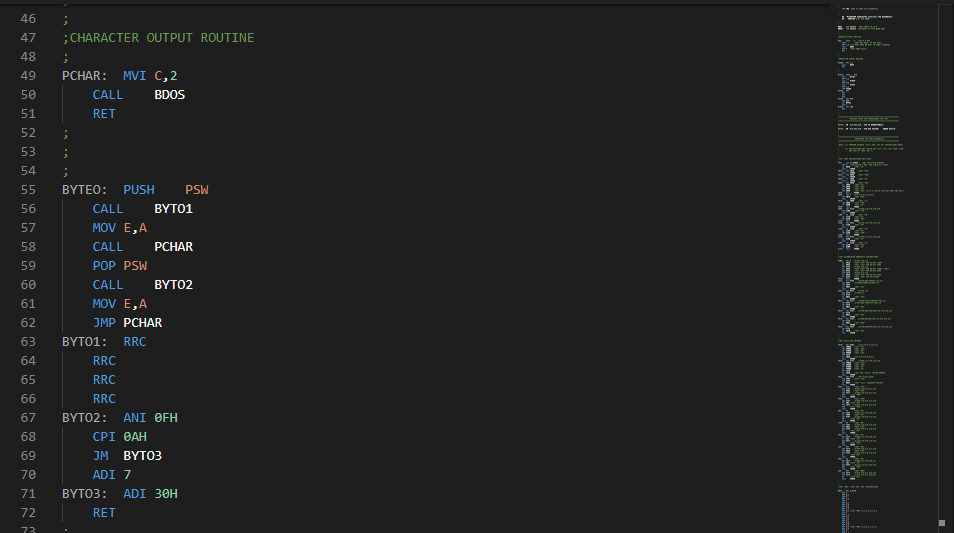
\includegraphics[width=1.0\textwidth]{Bilder/CodeEditor.png}
    \label{fig:codeeditor}
\end{figure}

In Abbildung \ref{fig:codeeditor} sieht man den Code-Editor in Aktion. Die einzelnen Bestandteile des Assembly-Codes, die Labels, die Instruktionen und die Argumente, sowie Kommentare sind alle unterschiedlich eingefärbt.

\begin{figure}
    \caption{Autovervollständigung für Instruktionen}
    \centering
    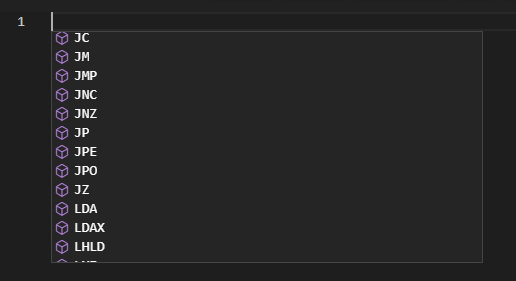
\includegraphics[width=0.6\textwidth]{Bilder/Completion1.png}
    \label{fig:completion1}
\end{figure}

In Abbildung \ref{fig:completion1} sieht man außerdem, wie die Autovervollständigung des Code-Editors funktioniert. Basierend auf der Eingabe des Nutzers und der Position im Code wird automatisch erkannt, ob eine Instruktion oder ein Argument vorgeschlagen werden soll und welche in Frage kommen.

\subsection{Emulator-Zustand}

Hat der Nutzer nun ein Assembly-Programm mithilfe des Code-Editors erstellt, kann er es ausführen. Hierfür wird der in Rust entwickelte Emulator genutzt, der mithilfe der \ac{WASM}-Schnittstelle in die Webapplikation eingebunden wird. Die Interaktion mit dem Emulator erfolgt mithilfe verschiedener Bedienelemente in einer Aktionsleiste am oberen Rand der Anwendung (siehe Abbildung \ref{fig:actionbar}).

\begin{figure}[h]
    \caption{Aktionsleiste des Emulators}
    \centering
    
\includegraphics[width=0.75\textwidth]{Bilder/Aktionsleiste.png}
    \label{fig:actionbar}
\end{figure}

\begin{figure}
    \caption{\textit{Load}-Dialog}
    \centering
    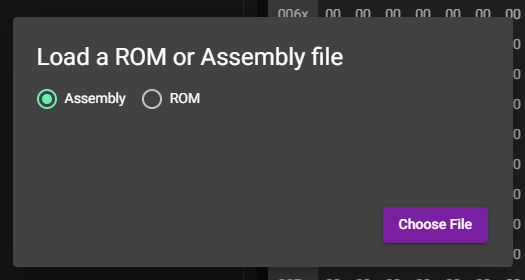
\includegraphics[width=0.75\textwidth]{Bilder/LoadDialog.png}
    \label{fig:loaddialog}
\end{figure}

Die ersten beiden Schaltflächen der Aktionsleiste, \textit{Load} und \textit{Save}, ermöglichen dem Nutzer, Assemblycode aus Dateien von seinem Endgerät zu laden oder sie dort zu speichern. \textit{Load} kann außerdem auch bereits übersetzten Code direkt in den Speicher des Emulators laden. Die Auswahl erfolgt mithilfe eines eigenen Auswahldialogs, der in Abbildung \ref{fig:loaddialog} zu sehen ist. Wird ein fertiges Programm geladen, kann außerdem bestimmt werden, an welcher Stelle es im Arbeitsspeicher platziert werden soll. Dies ist notwendig, da viele Programme beispielsweise erwarten, dass sich der Einstiegspunkt an der Speicheradresse 256 befindet.

Um den Code, den der Nutzer geschrieben hat, nun zu assemblen, muss dieser in der Aktionsleiste die Funktion \textit{Assemble} nutzen. Ist der Vorgang erfolgreich, werden die Bytes, die der Assembler erzeugt, in den Hauptspeicher des Emulators geschrieben. Die Emulation kann jetzt mithilfe der grünen Schaltfläche gestartet werden. Da die CPU keinen festgelegten Endzustand hat, läuft dieser solange weiter, bis der Nutzer die Emulation wieder beendet, was mit dem roten Stop-Knopf möglich ist.

Um den Ablauf des Codes nachvollziehen zu können, bietet die Applikation die Möglichkeit, jederzeit den internen Status des Prozessors einzusehen. Hierzu existiert auf der rechten Hälfte der Webseite eine Matrix, die den Arbeitsspeicher repräsentiert, sowie eine Anzeige für jedes der Register (siehe Abbildung \ref{fig:cpustate}).

\begin{figure}
    \caption{Anzeigen für den CPU-Status}
    \centering
    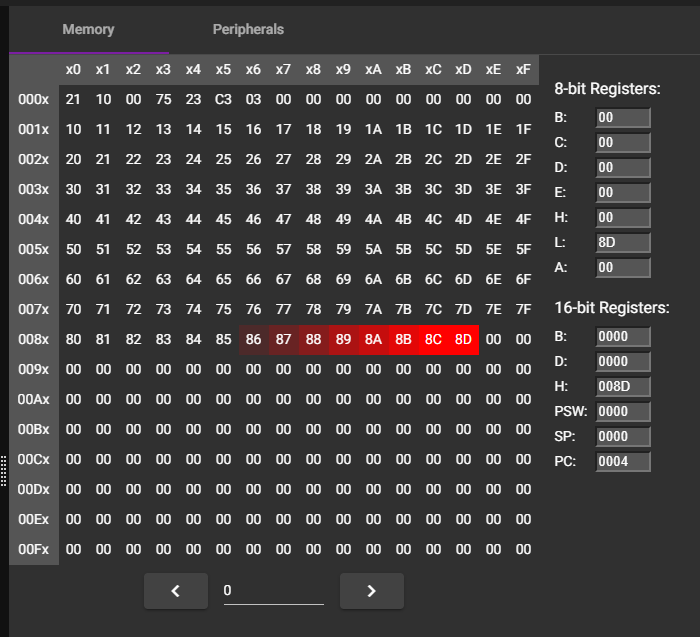
\includegraphics[width=0.75\textwidth]{Bilder/CPUState.png}
    \label{fig:cpustate}
\end{figure}

Die \ac{RAM}-Matrix stellt in jeder Zeile 16 Addressen dar, was die einfache Zuordnung von Zeile zu Spalte mithilfe der letzten Hexadezimalstelle erlaubt. Ändert sich im Arbeitsspeicher durch eine Instruktion des Prozessors ein Wert, wird dieser für eine kurze Zeit rot hinterlegt, um einfacher zu sehen, was sich geändert hat. Da der Speicher in der Regel deutlich größer ist, als die dargestellten 16x16 Bytes, nämlich bis zu 64KB, ist es möglich, den angezeigten Speicherbereich zu verschieben.

Die Registeranzeigen rechts von der \ac{RAM}-Matrix sind in zwei Kategorien gegliedert: Die 8-Bit Register (B, C, D, E, H, L, A) und die 16-Bit Register (BC, DE, HL, PSW, SP, PC).

Die aktuell ausgeführte Instruktion des Prozessors (basierend auf dem Program Counter) wird im Code-Editor außerdem rot hinterlegt. Für das Debugging von Programmen gibt es die Möglichkeit, die Ausführung des Emulators mithilfe der gelben Pause-Schaltfläche in der Aktionsleiste zu pausieren. Im pausierten Zustand kann nun jede Instruktion Schritt für Schritt ausgeführt werden.
\chapter{Implementierung}\label{chap:impl}

\section{Emulator}

\subsection{Registerarray}

Im folgenden werden drei Aspekte der Implementierungen des Registerarrays gezeigt: Die Repräsentation der Register, der Zugriff auf die Register und der Zugriff auf die Flaggen.

\subsubsection{Datentyp}

Naive Implementierungen eines Registerarrays würden die Register einzeln implementieren und für Registerpaare die entsprechenden Inhalte konkatenieren.
Dies ist jedoch unnötig umständlich. Der effizientere Ansatz ist die Register in Paaren zu speichern (als 16-Bit Unsigned Integer) und die Möglichkeit beizubehalten, die beiden Bytes individuell anzusprechen. In einer Sprache wie C ist dies mit Pointer-Arithmetik gut lösbar, in Rust ist es sinnvoller ein Union zu verwenden.

\begin{minted}{rust}
#[repr(C)]
union Register {
    bytes: (u8, u8),
    value: u16,
}
\end{minted}

Ein Union wird ähnlich wie ein Struct deklariert, jedoch teilen alle Felder den gleichen Speicherplatz\footnote{ausführliche Erklärung: \url{https://doc.rust-lang.org/reference/items/unions.html}}. Das bedeutet man kann den Wert eines solchen \rust{Register} entweder durch \rust{Register::bytes} als Tupel aus 2 Bytes oder durch \rust{Register::value} als 16-Bit-Wert auslesen. Dadurch ist keinerlei Konkatenation der Registerwerte notwendig.

\subsubsection{Registerzugriff}

Der Registerzugriff ist eine sehr häufig verwendete Operation, da ein großer Teil der zu implementierenden Instruktionen sie benötigt. Um dies möglichst einfach zu machen, wurde Indizierung für den Registerarray implementiert. Über String-Indizierung --- \rust{reg["bc"] // Registerpaar BC} --- ist Zugriff auf Registerpaare geregelt, über Character-Indizierung --- \rust{reg['b'] // Register B} --- der normale Zugriff.

\subsubsection{Flaggenzugriff}

Die Flags sind bekannterweise Teil des PSW-Registerpaars, sprich sie sind als einzelnes Byte gespeichert. Um die Werte der einzelnen Flaggen zu erhalten, werden Bitmasken verwendet. Um bspw. herauszufinden, ob das Bit mit dem höchsten Stellenwert gesetzt ist, muss der Ausdruck \rust{byte & 0x80 != 0} berechnet werden. Wenn dieser \rust{true} ist, ist das Bit gesetzt\footnote{\rust{0x80 == 0b10000000}}.

\subsection{Ein-/Ausgabegeräte}

In \cref{chap:design} ist zu sehen, dass die zentrale Struktur 2 Arrays mit 256 Elementen beinhaltet, um Ein- und Ausgabegeräte zu realisieren. Der Datentyp dieser Arrays wurde jedoch, der Übersichtlichkeit halber, vereinfacht. Das erste Problem eines solchen Arrays ist, dass initial keine Geräte registriert sind. Da es in Rust kein \rust{null} gibt, wäre das schlecht umsetzbar. Daher muss der \rust{Option}-Typ verwendet werden:

\rust{[Option<InputDevice>; 256]}

Hier ist jetzt jedoch problematisch, dass verschiedene Geräte registriert werden können. In klassischen objektorientierten Sprachen, wären Input- bzw OutputDevice hier Interfaces, in Rust arbeiten wir mit Traits (siehe \cref{chap:prereqs}). Da die Größe von Trait-Objekten nicht zur Compilezeit bestimmt werden kann, kann ein solches Objekt nicht auf dem Stack gelagert werden, daher muss ein Pointer verwendet werden. Rust verwendet sogenannte Smartpointer um die klassischen Probleme bei Verwendung von Pointern zu vermeiden. Meistens verwendet man hier \rust{Box}, jedoch erlaubt Box nicht, mehrere Referenzen auf die Daten zu haben. Dies brauchen wir jedoch, da sowohl von außen, als auch von innen mit den Geräten kommuniziert werden muss. Durch Kombination von \rust{Rc}, einem referenzzählendem Pointer, mit \rust{RefCell}, einer schreibbaren Speicherregion, kann das gewollte Verhalten erreicht werden. Die Syntax um einen derartigen Array zu deklarieren ist wie folgt:

\rust{[Option<Rc<RefCell<dyn InputDevice>>>; 256]}

Solange unser Programm single-threaded ist, kann nun jederzeit eine mutable-Referenz auf ein solches InputDevice erhalten werden und solange im aktuellen Scope keine mutable Referenz auf das Gerät existiert, können beliebig viele non-mutable Referenzen verwendet werden.

\chapter{Auswertung}\label{chap:eval}

\section{Testprogramme}

Ziel dieser Arbeit ist es, die komplette Spezifikation des Intel 8080 zu implementieren. Um zu überprüfen, ob dies tatsächlich gelungen ist, müssen Tests durchgeführt werden. Hierfür kommen frei verfügbare \footnote[1]{\url{https://altairclone.com/downloads/cpu_tests/}} CPU Testprogramme zum Einsatz, die die Funktionsweise verschiedener Instruktionen überprüfen und mit Sollzuständen vergleichen.


\chapter{Zukunftsideen}

Dieses Kapitel behandelt Ideen zur Erweiterung von \Emu.

\section{Dynamic Recompilation}

Bei Dynamic Recompilation handelt es sich um eine Optimierungsstrategie, bei der Maschinencode des emulierten Systems auf Maschinencode des ausführenden Systems übersetzt wird. In unserem Fall würde dabei Intel 8080 Maschinencode zu WebAssembly kompiliert werden. Diese Rekompilation findet zur Laufzeit statt.


\section{Intel Hex}

Momentan gibt der Assembler einen Vektor aus Bytes zurück, welcher in den RAM des Emulators geladen wird um ein Programm zu laden. Ein alternatives Format für die Assembler-Ausgabe wäre das Intel Hex-Format, ein Dateiformat um Binärdaten im ASCII-Format zu speichern. In Intel Hex repräsentiert jede Zeile einen Datensatz, der eine konsekutive Bytefolge enthält. Ein solcher Datensatz enthält 6 Felder:

\begin{enumerate}
\item Satzbeginn: ein ASCII Doppelpunkt am Anfang der Zeile
\item Anzahl an Bytes: Wie viele Datenbytes enthalten sind
\item Speicheradresse: 16-Bit Adresse im Speicher, an der der Datenblock beginnt
\item Datensatztyp: 00..05
\item Daten: n Bytes (als 2n Hex-Zeichen kodiert)
\item Prüfsumme: 2 Hex-Zeichen große Prüfsumme über den Datensatz
\end{enumerate}

Dieses Format zu verwenden hat den Vorteil, leere Regionen zwischen Assembly Instruktionen nicht abspeichern zu müssen. Außerdem sind ROMs für den 8080 häufig in diesem Format vorliegend, daher wäre es sinnvoll solche Dateien einlesen zu können.


\begin{appendices}
\renewcommand{\appendixtocname}{Anhänge}
\chapter{Anhang}
Jeglicher Code, der im Verlauf dieser Arbeit entwickelt und vorgestellt wurde, ist öffentlich auf GitHub zugänglich: 


\url{https://github.com/moorts/name_is_wip}
\medskip

\noindent
Zum Zeitpunkt der Veröffentlichung wird mittels GitHub Pages die aktuellste Version des Emulators auf einer zusätzlichen Webseite deployed: 

\url{https://moorts.github.io/name_is_wip/}
\medskip

\noindent
Die Weboberfläche basiert zu großen Teil auf zwei Open Source Projekten:

\begin{itemize}
	\item Angular: \url{https://angular.io/}
	\item Monaco Editor: \url{https://microsoft.github.io/monaco-editor/}
\end{itemize}

\end{appendices}

\renewcommand{\thepage}{\Roman{page}}
\printbibliography

\end{document}
